% compile with: pdflatex -shell-escape filename.tex
\documentclass[crop,tikz,convert=pdf2svg]{standalone}
\usetikzlibrary{arrows}
\usetikzlibrary{backgrounds}

\begin{document}

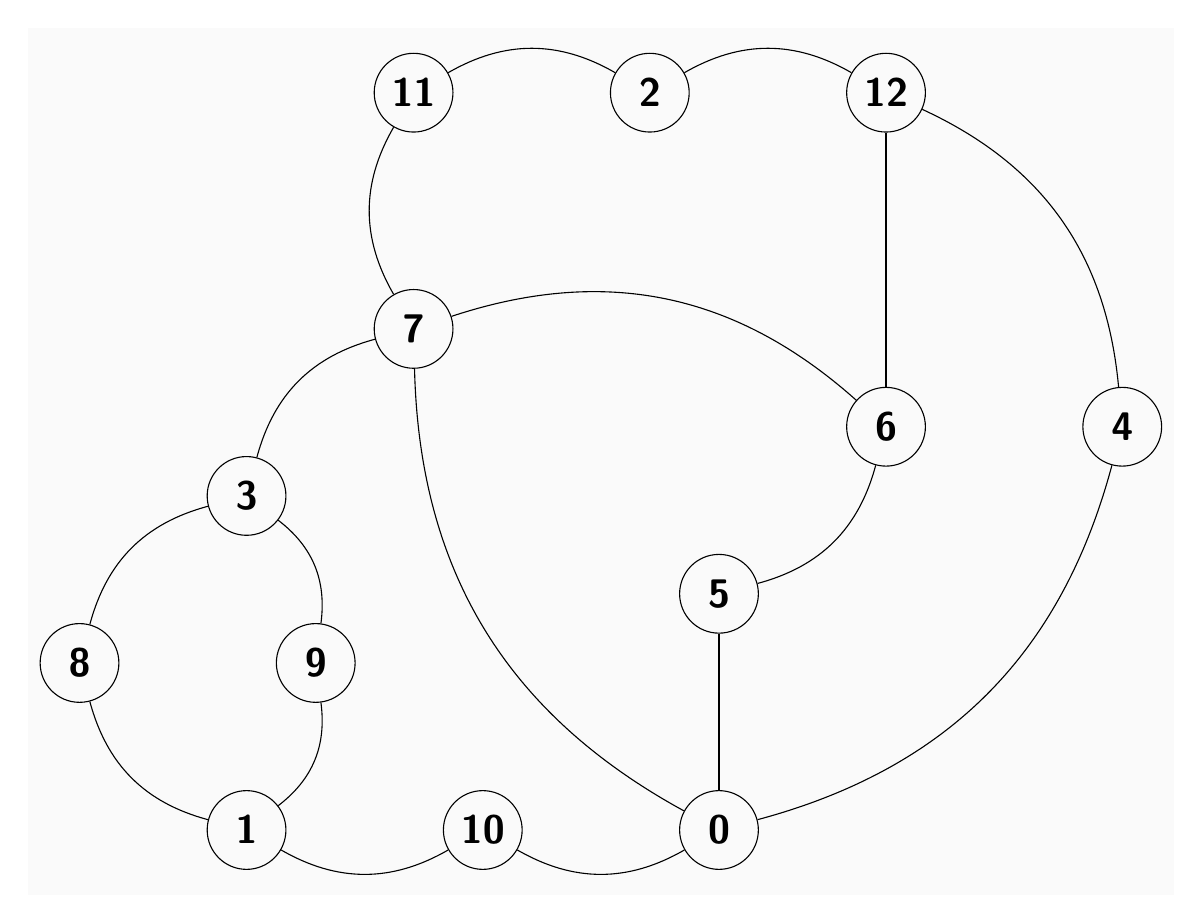
\begin{tikzpicture}[
    background rectangle/.style={fill=black!02},
    show background rectangle,
    node distance=3cm,
    main node/.style={circle,draw,font=\sffamily\Large\bfseries,minimum size=1cm},
  ]

  \node[main node] (8) {8};
  \node[main node] (3) [above right of=8] {3};
  \node[main node] (9) [right of=8] {9};
  \node[main node] (1) [below right of=8] {1};
  \node[main node] (7) [above right of=3] {7};
  \node[main node] (10) [right of=1] {10};
  \node[main node] (11) [above of=7] {11};
  \node[main node] (2) [right of=11] {2};
  \node[main node] (12) [right of=2] {12};
  \node[main node] (0) [right of=10] {0};
  \node[main node] (5) [above of=0] {5};
  \node[main node] (6) [above right of=5] {6};
  \node[main node] (4) [right of=6] {4};

  \path[every node/.style={font=\sffamily\small}]
  (8) edge [bend right] (1)
  (8) edge [bend left] (3)
  (9) edge [bend left] (1)
  (9) edge [bend right] (3)
  (1) edge [bend right] (10)
  (10) edge [bend right] (0)
  (3) edge [bend left] (7)
  (7) edge [bend right] (0)
  (7) edge [bend left] (11)
  (11) edge [bend left] (2)
  (2) edge [bend left] (12)
  (7) edge [bend left] (6)
  (0) edge (5)
  (5) edge [bend right] (6)
  (6) edge (12)
  (0) edge [bend right] (4)
  (4) edge [bend right] (12)
  ;
\end{tikzpicture}
\end{document}
